\section{FlakyCat}
\label{sec:flakycat-flakycat}

\begin{figure}[htbp]
\centering
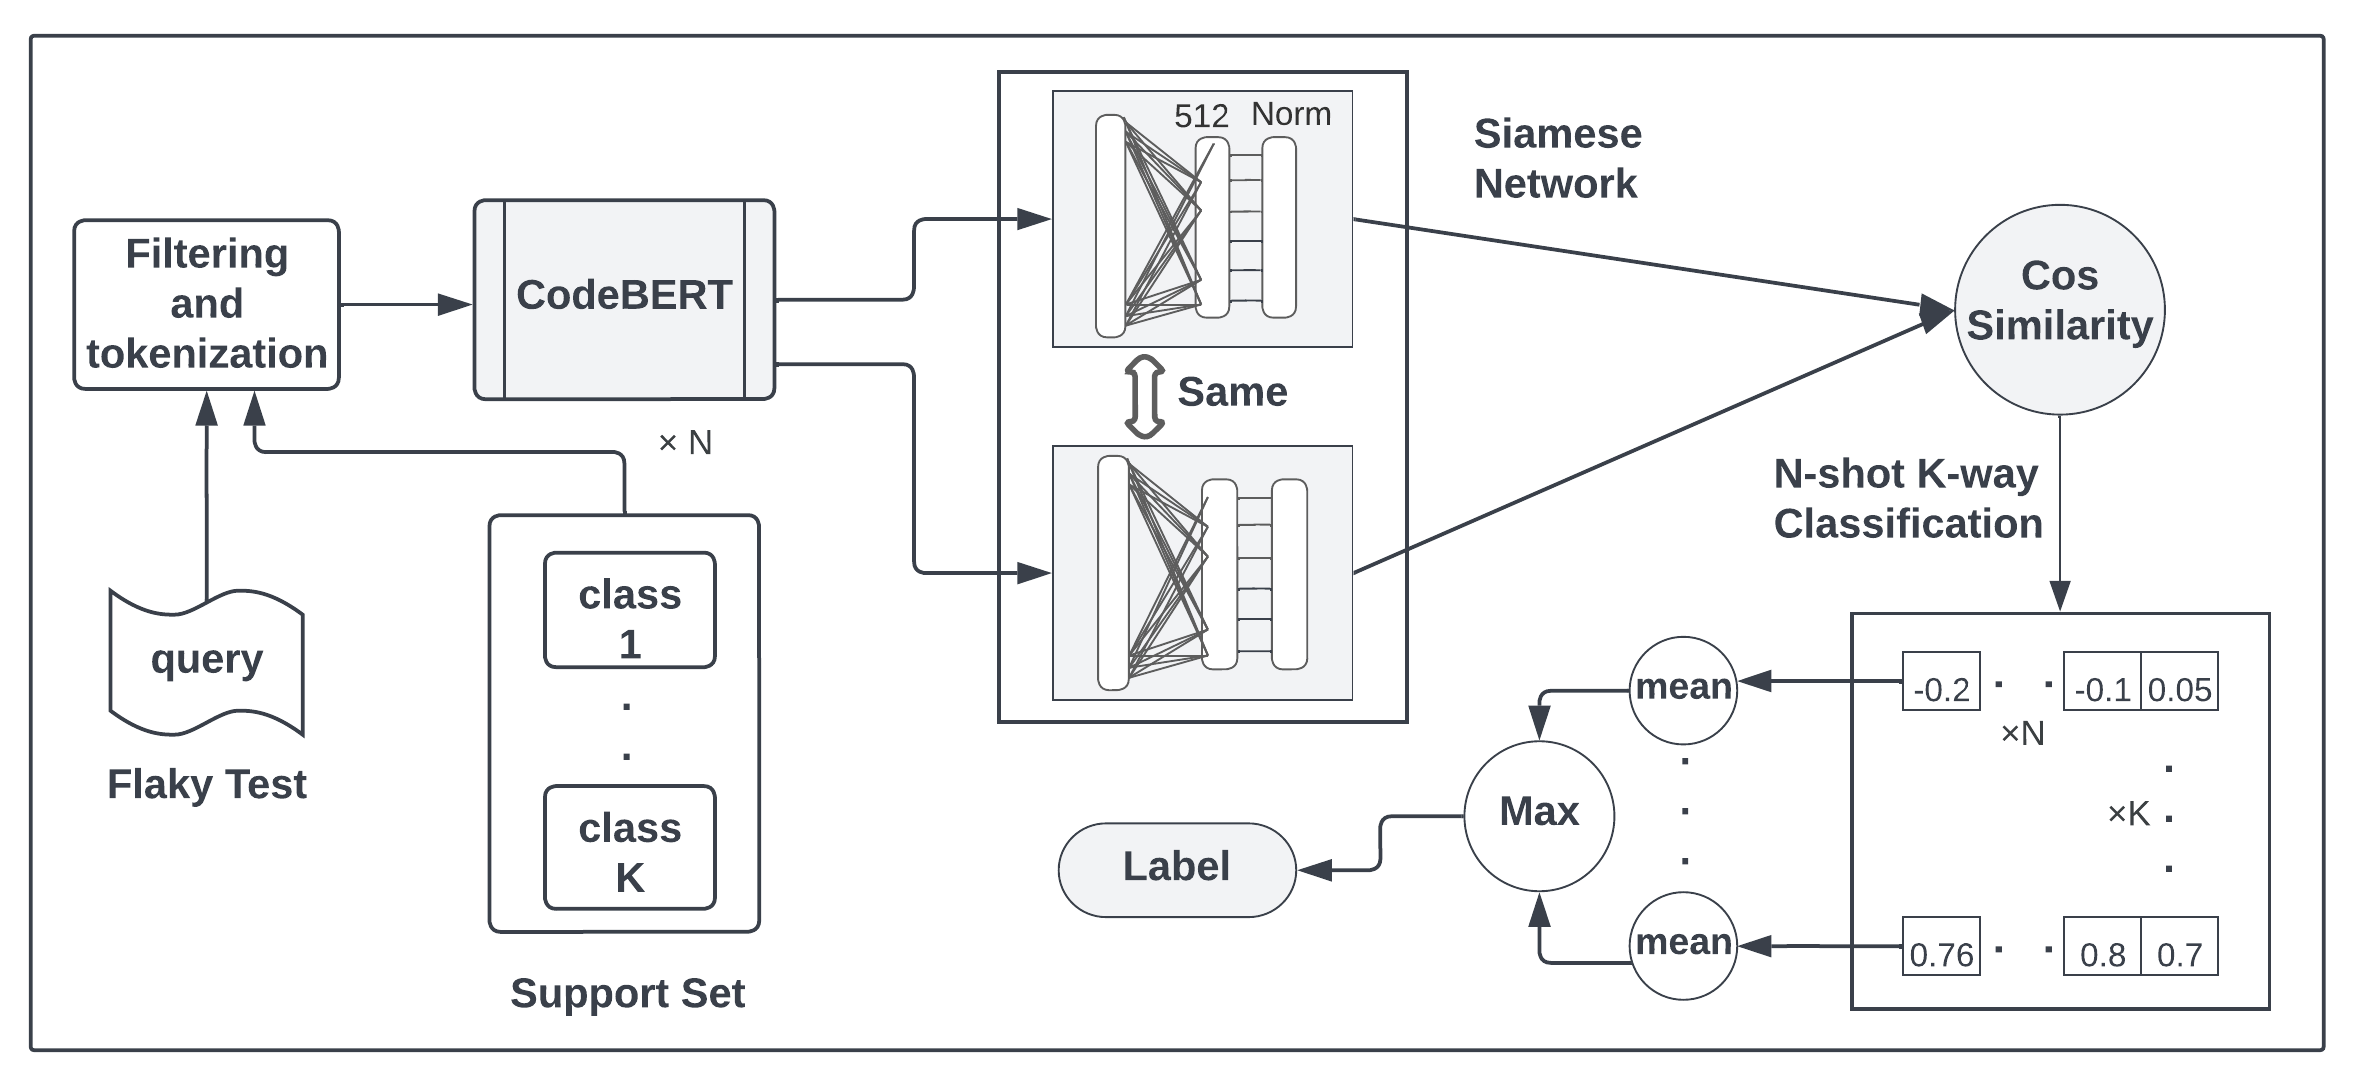
\includegraphics[width=0.8\textwidth,scale=1]{figures/flakycat/architecture.png}
\caption{An overview of FlakyCat, which combines the use of the pre-trained model CodeBERT, and Few Shot Learning based on the Siamese network.}
\label{fig:general_arch}
\end{figure}

In this section, we present the design and implementation of our approach.
Figure~\ref{fig:general_arch} presents an overview of the main steps of FlakyCat, code transformation and classification. 

\subsection{Step 1: Flaky Test Transformation}

\subsubsection{Scope} We rely on the test code to assign flaky tests to different categories.
Previous studies showed that flakiness finds its root causes in the test in more than 70\% of the cases\cite{Luo2014,Lam2020a}. 
Hence, focusing on the test code allows us to capture the nature of flakiness while minimizing the overall cost of FlakyCat. 
Indeed, considering the code under test would require running the tests and collecting the coverage, which entails additional requirements and costs.

\subsubsection{Flaky Test Vectorization}
In order to perform a source code classification task, we first need to transform the code into a suitable representation that will be fed to the classification model. Among previous studies predicting flaky tests statically, two main approaches were used to transform code into vectors: using test smells~\cite{camara2021use,FlakeFlagger} and using code vocabulary \cite{Pinto2020,Haben2021,Camara2021VocabExtendedReplication}.
Both approaches seem promising, as different studies report high-performance models. As their encoding enables flaky test prediction, we believe they could also be used for flakiness category prediction, and we compare them with our approach. 

Recently, code embeddings from pre-trained language models were also considered for source code representation~\cite{fatima2021flakify,zhou2021assessing}. Pre-trained language models allow the encoding of code semantics and are intended for general-purpose tasks such as code completion, code search, and code summarization.
Considering these benefits, we use the pre-trained language model CodeBERT \cite{feng-etal-2020-codebert} to generate source code embeddings. 
CodeBERT can learn the syntax and semantics of the code and doesn't require any predefined features \cite{wan2022they}. Considering this aspect, we decide to rely on the CodeBERT test representation.

CodeBERT has been developed with a multi-layer transformer architecture~\cite{transformer} and trained on over six million pieces of code involving six programming languages (Java, Python, JavaScript, PHP, Ruby, and Go). 

To get the code representation using CodeBERT model, we first filter out extra spaces such as line breaks and tabs from the source code. In our case, we use each test method's source code as individual sequences. We then tokenise sequences by converting each token into IDs. Each sequence is passed to the CodeBERT model, which returns a vector representation. Figure~\ref{fig:using_codebert} illustrates this process.

Next, we explain the inputs and outputs of CodeBERT.

\paragraph{Inputs}
CodeBERT is able to process both source code and natural language, \eg comments and documentation. In our case, we did not exploit the possibility of using comments as the input length of CodeBERT is limited. Furthermore, comments can add noise since they represent unstructured text, possibly written by different developers, so we decided to solely rely on the code semantics. 
Hence, the given input to CodeBERT only considers code tokens, surrounded by two special tokens for boundaries. This is represented as follows: 
\begin{center}
 \([CLS], c1, c2, ..., cm, [SEP]. \)
\end{center}
Where \textit{Ci} is a sequence of code tokens, the special token [SEP] indicates the end of the sequence, and [CLS] is a special token placed in the beginning, whose final representation is considered as the representation of the whole sequence which we use for classification.

\paragraph{Outputs}

CodeBERT output includes two representations. The first one is the context matrix where each token is represented by a vector, and the second one is the CLS representation, having a size of 768, which is an aggregation of the context matrix and represents the whole sequence.
For the purpose of FlakyCat, we are interested in the CLS vector that represents the complete test code.

\begin{figure}[htbp]
\centering
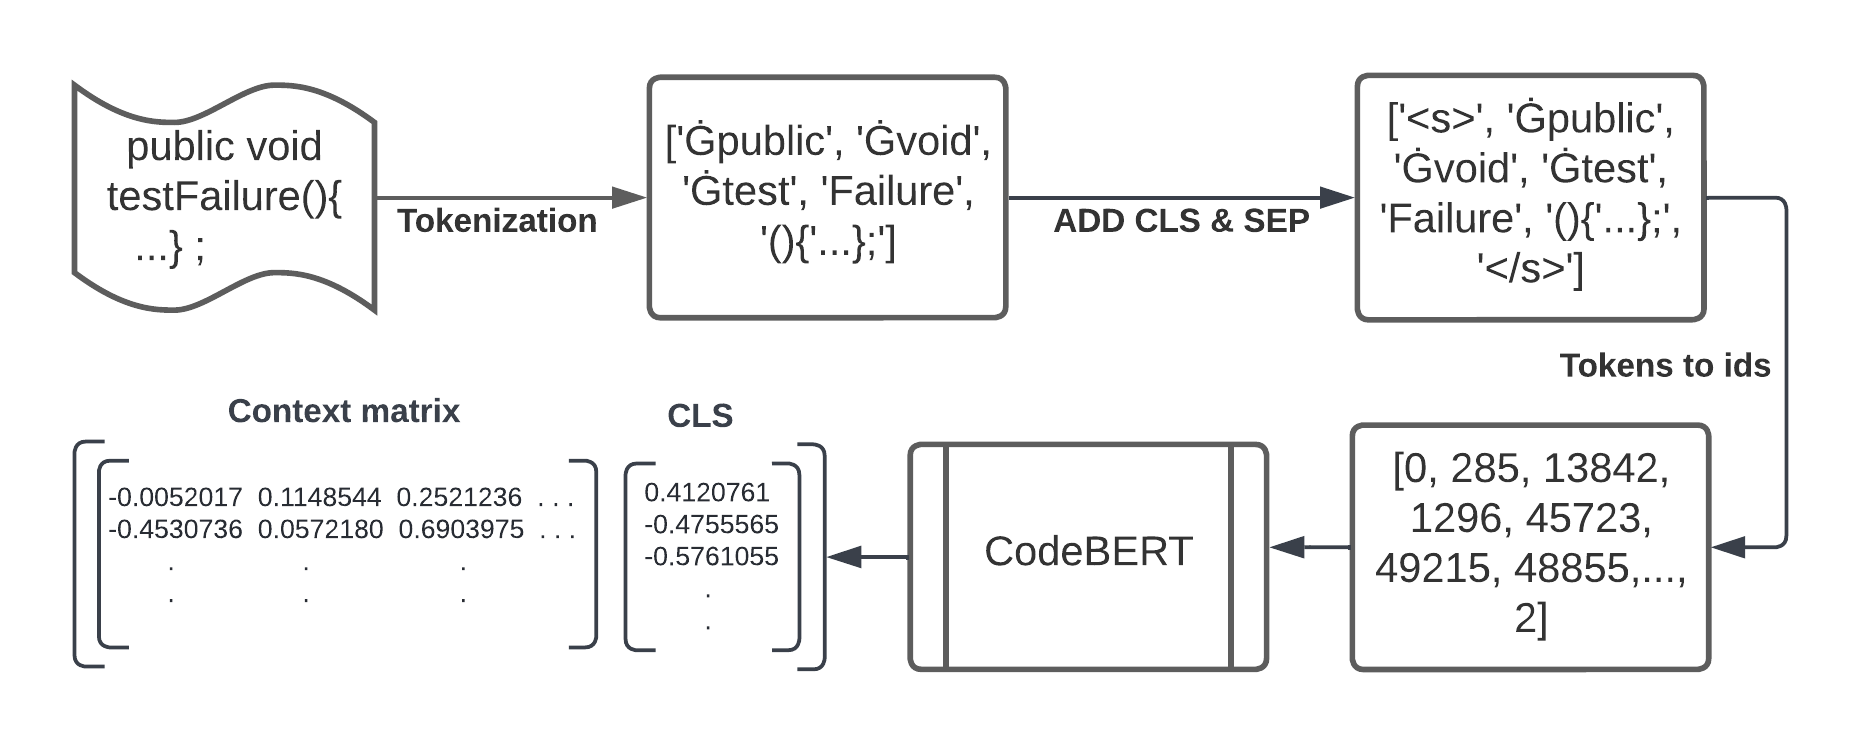
\includegraphics[width = 0.8\textwidth, scale=1]{figures/flakycat/codebert_transform.png}
\caption{The process of converting the source code of each test case to a vector using CodeBERT, going through tokenization, then converting to IDs and applying the CodeBERT model to get the representation (CLS vector). Ǵ represent spaces, $<s>$ used for CLS, and $</s>$ for SEP. }
\label{fig:using_codebert}
\end{figure}

\subsection{Step 2: Flaky Test Categorization}

\subsubsection{Classification process}

Unlike traditional machine learning classifiers that attempt to learn how to match an input $x$ to a probability $y$ by training the model in a large training dataset and then generalizing to unseen examples, Few-Shot Learning (FSL) classifiers learn what makes the elements similar or belonging to the same class from only a few data. Facing the scarcity of data on flaky tests, selecting an FSL classifier seems then to be a promising choice. 

In FSL, we call the item we want to classify a \textit{query}, and the \textit{support set} is a small set of data containing few examples for each class used to help the model to make classifications based on similarity as shown in Figure~\ref{fig:general_arch}.
To classify flaky tests according to their flakiness category, we compute the similarity between the query and all examples of each flakiness category in our Support Set and assign the label having the maximum similarity with the query. This classification is obviously performed in a space where all elements of the same class are similar or close to each other. This is achieved by a model called \textit{Siamese network}. Its task is to transform the data and project it into a space where all the elements of a same class are close to each other, and then to classify the elements by computing their similarity.

The Siamese network has knowledge of the similarity of elements of the same class. It processes two vectors in input and applies transformations that allow minimizing the distance between the two vectors if they share similar characteristics. Figure~\ref{fig:before_after} shows an example of the visualization of flaky test vectors before and after the Siamese network is applied. Since CodeBERT has no knowledge of the characteristics of flaky tests and only generates a general representation of the source code, the vectors produced are all similar.
However, the Siamese networks learn which characteristics in these vectors are shared by tests of the same class, and thus allow to project vectors into a space that groups tests of the same flakiness category. After this step, it becomes possible to classify them using a similarity computation.

\begin{figure}[htbp]
\centering
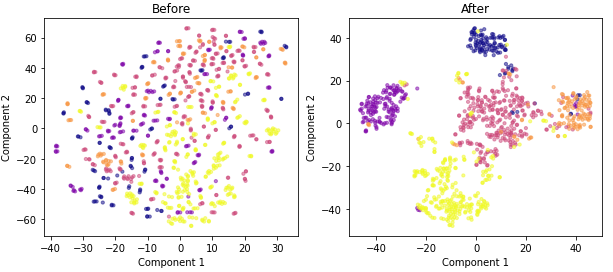
\includegraphics[width = 0.8\textwidth, scale=1]{figures/flakycat/before_after.PNG}
\caption{Visualization of our data before and after training of the Siamese network with the triplet loss, which brings together the elements of the same class.}
\label{fig:before_after}
\end{figure}

\subsubsection{Model training}

Siamese networks have two identical sub-networks, each sub-network processes the input vector and performs transformations.
Both sub-networks are trained by calculating the similarity between the two inputs and using the similarity difference as a loss function.
Accordingly, the weights are adjusted to have a high similarity if the inputs belong to the same class. For the architecture of the sub-networks, we used a dense layer of 512 neurons and a normalization layer as shown in Figure~\ref{fig:general_arch}.
We also performed a linear transformation to keep relations learnt by CodeBERT using the attention mechanism introduced in the transformer architecture \cite{transformer}. 
This model is trained using a Triplet Loss function, based on the calculation of similarity difference.

Let the Anchor $A$ be the reference input (it can be any input), the positive example $P$ is an input that has the same class as the Anchor, the negative example $N$ is an input that has a different class than the Anchor, $s()$ is the cosine similarity function, and $m$ is a fixed margin. The idea behind the Triplet Loss function is that we maximize the similarity between $A$ and $P$, and minimize the similarity between $A$ and $N$, so ideally $s(A, P)$ is large and $s(A, N)$ is small. The formula for this loss function is: 

\begin{center}
\( Loss = max(s(A, N) - s(A, P) + m, 0) \)
\end{center}

$m$ is an additional margin as we do not want $s(A, P)$ to be very close to $s(A, N)$, which would lead to a zero loss. 

To train the Siamese network with the triplet loss, we give as input batches of pairs with the same classes, and any other pair of a different class can be used as a negative example. We select the closest negative example to the anchor, such as $s(A,  N)$ $\simeq$ $s(A, P)$, which generates the largest loss and constitutes a challenge for model learning. 